\documentclass[12pt]{article}
\usepackage{amsfonts, amsmath, amssymb, bm}
\usepackage{dcolumn, multirow}
\usepackage{subfigure, subfloat, graphicx, float}
\usepackage{anysize, setspace}
\usepackage{verbatim, rotating, paralist}
\usepackage[format=hang]{caption}[2006/03/21]
\usepackage{natbib,url}
\setdefaultenum{I)}{A)}{i.}{a.}
\singlespace
\bibpunct[, ]{(}{)}{,}{a}{}{,}
\newcommand{\mc}[1]{\multicolumn{1}{c}{#1}}
\newcommand{\R}{\textbf{R }}
\pagestyle{myheadings}
\newcolumntype{d}[1]{D{.}{.}{#1}}
\usepackage[top=1in, bottom=1in, left=1.5in, right=1in]{geometry}
\usepackage{lipsum}
\renewcommand{\contentsname}{\centerline{TABLE OF CONTENTS}}
\renewcommand{\listfigurename}{\centerline{LIST OF FIGURES}}
\renewcommand{\listtablename}{\centerline{LIST OF TABLES}}
\makeatletter
\renewcommand\section{\@startsection {section}{1}{\z@}%
                                   {-3.5ex \@plus -1ex \@minus -.2ex}%
                                   {2.3ex \@plus.2ex}%
                                   {\normalfont\scshape\bfseries\LARGE}}
\makeatother

%%%%%%%%%%%%%%%%%%%%%%%%%%%%%%%%%%%%%%%%%%
% THIS TEMPLATE WAS CREATED BY MICHAEL A. HANSEN WITH THE INTENT THAT OTHER GRADUATE SCHOOL STUDENTS WOULD USE OR ALTER THE CONTENTS FOR FORMATTING A UW-MILWAUKEE PHD DISSERTATION  %
%%%%%%%%%%%%%%%%%%%%%%%%%%%%%%%%%%%%%%%%%%


\begin{document}
% The command below sets the bibliography style as American Political Science Review (APSR) style.
\bibliographystyle{apsr}
\doublespacing
\thispagestyle{empty}

%%%%%%%%%%%%%%%%%%%%%%%%%%%%%%%%%%%%%%%%%%
%% %%%%%%%%  TITLE PAGE  %%%%%%%%%%%%%%
%%%%%%%%%%%%%%%%%%%%%%%%%%%%%%%%%%%%%%%%%%
\begin{center}
THE TITLE GOES HERE AND MUST BE IN ALL CAPS AND THE TEXT MUST BE DOUBLE SPACED
\end{center}

\begin{center}
by\\
\end{center}

\begin{center}
Author Name\\
\end{center}

\begin{center}
A Dissertation Submitted in\\
Partial Fulfillment of the\\
Requirements for the Degree of\\
\end{center}

\begin{center}
Doctor of Philosophy\\
in Political Science\\
\end{center}

\begin{center}
at\\
University of Wisconsin-Milwaukee\\
May 2016
\end{center}

%%%%%%%%%%%%%%%%%%%%%%%%%%%%%%%%%%%%%%%%%%
%% %%%%%%%%  ABSTRACT PAGE  %%%%%%%%%%%%%%
%%%%%%%%%%%%%%%%%%%%%%%%%%%%%%%%%%%%%%%%%%
\newpage
\thispagestyle{plain}

\singlespacing
\begin{center}
ABSTRACT\\
THE TITLE OF THE DISSERTATION IS REPEATED HERE, BUT THIS TIME IT IS SINGLE SPACED
\end{center}

\doublespacing
\begin{center}
by\\
\end{center}

\begin{center}
Author Name\\
\end{center}

\singlespacing
\begin{center}
The University of Wisconsin-Milwaukee, 2016\\
Under the Supervision of Professor name of major professor\\
\end{center}

\doublespacing
\noindent
Abstract text goes here. Remember to double space, and left-justify the text.
March, 2013 ProQuest states: We no longer have a word limit on your abstract, as this constrains your ability to describe your research in a section that is accessible to search engines, and therefore would constrain potential exposure of your work. However, we continue to publish print indexes that include citations and abstracts of all dissertations and theses published by ProQuest/UMI. These print indexes require limits of 350 words for doctoral dissertations and 150 words for master's theses. Additionally, our print indexes allow only text to be included in the abstract. In the editorial process for these print publications, we will simply truncate your abstract if it exceeds these word limits and remove any non-text content. You may wish to limit the length of your abstract if this concerns you. The abstract as you submit it will NOT be altered in your published manuscript. Please include an additional version of your abstract in English, even if the primary language of your dissertation or thesis is NOT English.
%The command below sets the bags number to lower case roman numerals.
\renewcommand{\thepage}{\roman{page}}

%%%%%%%%%%%%%%%%%%%%%%%%%%%%%%%%%%%%%%%%%%
%% %%%%%%%%  COPYRIGHT  PAGE  %%%%%%%%%%%%%%
%%%%%%%%%%%%%%%%%%%%%%%%%%%%%%%%%%%%%%%%%%
\newpage
\thispagestyle{plain}

% Centering commands.
\null\vfill
\begin{center}
\copyright \ by Author Name, 2016\\
All Rights Reserved
\end{center}
\vfill\null

%%%%%%%%%%%%%%%%%%%%%%%%%%%%%%%%%%%%%%%%%%
%% %%%%%%%%  TABLE OF CONTENTS  %%%%%%%%%%%%%%
%%%%%%%%%%%%%%%%%%%%%%%%%%%%%%%%%%%%%%%%%%

\newpage
\thispagestyle{plain}

% The command below automatically adds sections to the table of contents.
\tableofcontents

%%%%%%%%%%%%%%%%%%%%%%%%%%%%%%%%%%%%%%%%%%
%% %%%%%%%%  LIST OF FIGURES  %%%%%%%%%%%%%%
%%%%%%%%%%%%%%%%%%%%%%%%%%%%%%%%%%%%%%%%%%
\newpage
\thispagestyle{plain}

% The command below automatically adds figures to the "list of figures" once included in the body of the text.
\addcontentsline{toc}{section}{List of Figures}
\listoffigures





%%%%%%%%%%%%%%%%%%%%%%%%%%%%%%%%%%%%%%%%%%
%% %%%%%%%%  LIST OF TABLES  %%%%%%%%%%%%%%
%%%%%%%%%%%%%%%%%%%%%%%%%%%%%%%%%%%%%%%%%%
\newpage
\thispagestyle{plain}

% The command below automatically adds tables to the "list of tables" once included in the body of the text.
\addcontentsline{toc}{section}{List of Tables}
\listoftables

%%%%%%%%%%%%%%%%%%%%%%%%%%%%%%%%%%%%%%%%%%
%% %%%%%%%%  LIST OF ABBREVIATIONS  %%%%%%%%%%%%%%
%%%%%%%%%%%%%%%%%%%%%%%%%%%%%%%%%%%%%%%%%%
\newpage
\thispagestyle{plain}

\addcontentsline{toc}{section}{List of Abbreviations}
\begin{center}
LIST OF ABBREVIATIONS\\
\end{center}

\singlespacing
\noindent
GSF - Graduate School Freakout\\
GSW - Graduate School Work

%%%%%%%%%%%%%%%%%%%%%%%%%%%%%%%%%%%%%%%%%%
%% %%%%%%%%  ACKNOWLEDGEMENTS  %%%%%%%%%%%%%%
%%%%%%%%%%%%%%%%%%%%%%%%%%%%%%%%%%%%%%%%%%
\newpage
\thispagestyle{plain}

\begin{center}
ACKNOWLEDGEMENTS\\
\end{center}

\noindent
The author would like to thank all of the members of their dissertation committee, etc.
%The command below auto-fills text. Delete the command to remove the fake text
\lipsum[3-4]

%%%%%%%%%%%%%%%%%%%%%%%%%%%%%%%%%%%%%%%%%%
%% %%%%%%%%  START OF SECTIONS  %%%%%%%%%%%%%%
%%%%%%%%%%%%%%%%%%%%%%%%%%%%%%%%%%%%%%%%%%


\newpage
% The command below enters the chapter name into the "table of contents."
\addcontentsline{toc}{section}{Chapter 1 - The Name of the Chapter}
\section*{Chapter 1 \\
\begin{flushright}
 The Name of the Chapter
 \end{flushright}}
% The two command below sets the page numbering to Arabic and sets the current page to page 1.
\renewcommand{\thepage}{\arabic{page}}
\setcounter{page}{1}
%The space command sets the space between the text above and the text below.. 
\vspace{4cm}

This is how you cite \citep{Hansen2014}. \citet{Hansen2014} says there are many ways to cite in a paper. Hansen's \citeyearpar{Hansen2014} template offers many opportunities to do this task. However, the BibDesk reference software is needed first. \\

% Sample table. The name entered after the caption command is auto-filled into the "list of tables" as the table name.  Any table made using the tabular environment will appear in the "list of tables", which includes the page number of the table.
\begin{table}[ht]
\caption{Sample Table}
\begin{center}
\begin{tabular}{|lcc|}
  \hline
Answer & \# of Respondents & \% of Respondents \\ 
  \hline
Agree & 81 & 16.50\\ 
  No opinion & 270 & 54.99 \\ 
  Disagree & 140 & 28.51\\ 
   \hline
\end{tabular}
\end{center}
\end{table}

%The command below auto-fills text. Delete the command to remove the fake text. 
\lipsum






\newpage
\addcontentsline{toc}{section}{Chapter 2 - Chapter Name}
\section*{Chapter 2 \\
\begin{flushright}
 Chapter Name
 \end{flushright}}
 \vspace{4cm}

% Sample figure. The name entered after the caption command is auto-filled into the "list of figures" as the figure name. To include a figure. Save a figure as a pdf, then in the include graphics line enter the figure name after the dimensions specification (ex. FigureName)
\begin{figure}[ht]
\begin{center}
 \caption{Sample Figure}
 \vspace{-.5cm}
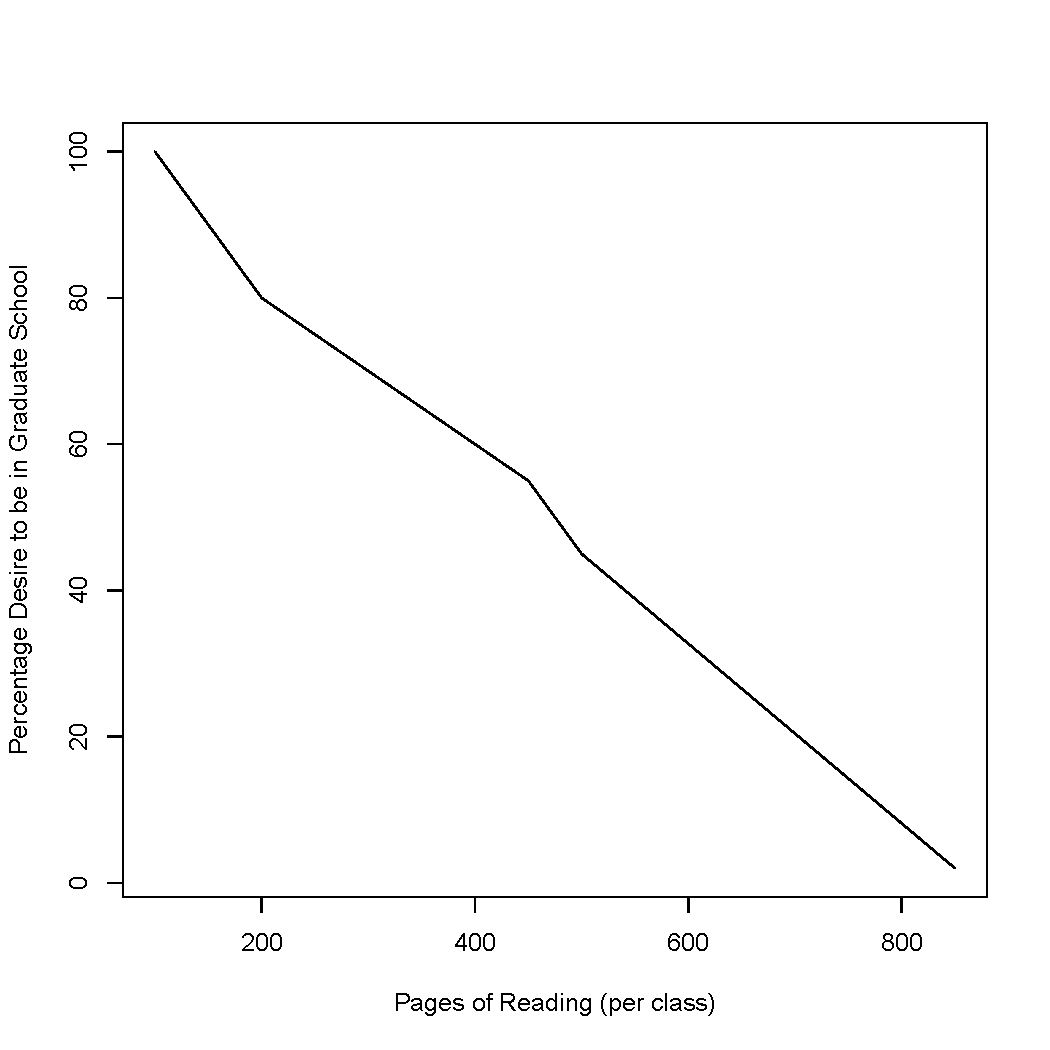
\includegraphics[height=4in, width=4.5in]{FigureName}
\end{center}
\end{figure}

%The command below auto-fills text. Delete the command to remove the fake text. 
\lipsum






\newpage
\addcontentsline{toc}{section}{Chapter 3 - Chapter Name}
\section*{Chapter 3 \\
\begin{flushright}
 Chapter Name
 \end{flushright}}
 \vspace{4cm}

%The command below auto-fills text. Delete the command to remove the fake text. 
\lipsum






\newpage
\addcontentsline{toc}{section}{Chapter 4 - Chapter Name}
\section*{Chapter 4 \\
\begin{flushright}
 Chapter Name
 \end{flushright}}
 \vspace{4cm}

%The command below auto-fills text. Delete the command to remove the fake text. 
\lipsum




\newpage
\addcontentsline{toc}{section}{Chapter 5 - Chapter Name}
\section*{Chapter 5 \\
\begin{flushright}
 Chapter Name
 \end{flushright}}
 \vspace{4cm}

%The command below auto-fills text. Delete the command to remove the fake text. 
\lipsum


\newpage
\addcontentsline{toc}{section}{Chapter 6 - Chapter Name}
\section*{Chapter 6 \\
\begin{flushright}
 Chapter Name
 \end{flushright}}
 \vspace{4cm}

%The command below auto-fills text. Delete the command to remove the fake text. 
\lipsum




\newpage
% Once the bibliography is saved as the name "bibdesk". As long as you put the bibliography into the same folder the command below will automatically enter in all of your references. You must typeset "latex", then  typeset "BibTex", then typeset "latex" twice again for citations to show up in the text and reference section.
\addcontentsline{toc}{section}{References}
\bibliography{bibdesk}

\newpage
\addcontentsline{toc}{section}{Appendix}
\section*{Appendix}




\end{document}




